\chapter{Implementation} \label{Implementation}

Pequeno rundown de como vamos a estar haciendo las varas.

For the creation of such a testing environment, four elements were recognized as of utmost importance to the validity of the tests and the author sought to implement them accordingly. In the following, they will be presented with detail, justifying the sources of the models and the parameter choices made.

The aforementioned elements are:

\begin{itemize}
	\item Generation and distribution of UEs %\ref{PPP}
	\item Path loss (attenuation) %\ref{PL}
	\item Shadow fading %\ref{SF}
	\item Random access procedure and interference %\ref{RAP}
  \item Clustering algorithms
\end{itemize}

\section{Generation and distribution of UEs} \label{PPP}
Often called a ``completely'' random process, a Poisson process is a process where every event is stochastically independent of all other points in it, see \cite{Keeler2016}. This generation process is common in investigations about the performance of networks, as eloquently expressed by \cite{Keeler} In our case, the Poisson-distributed random variable are the number of points in the bounded region we are investigating. The distribution is described by the following probability mass function:

\begin{equation} \label{eq:Poisson}
P\left( x\ points\ in\ region \right) = \frac{{e^{ - \lambda } \lambda ^x }}{{x!}}
\end{equation}

By providing the $\lambda$ above, often called mean density (\cite{Keeler2016}), we can adjust the expected amount of points generated in a given area. In order to evaluate the robustness of different algorithms, the tests were made with a variety of $\lambda$ values. The generated amount of points are then distributed in the given area with a uniform distribution, where both the $x$ and $y$ value are distributed along the appropriate axis. In both cases, the \textit{Python} package \textit{NumPy} was utilized for the realization of the random distributions.

\begin{figure}[!h]
\centering
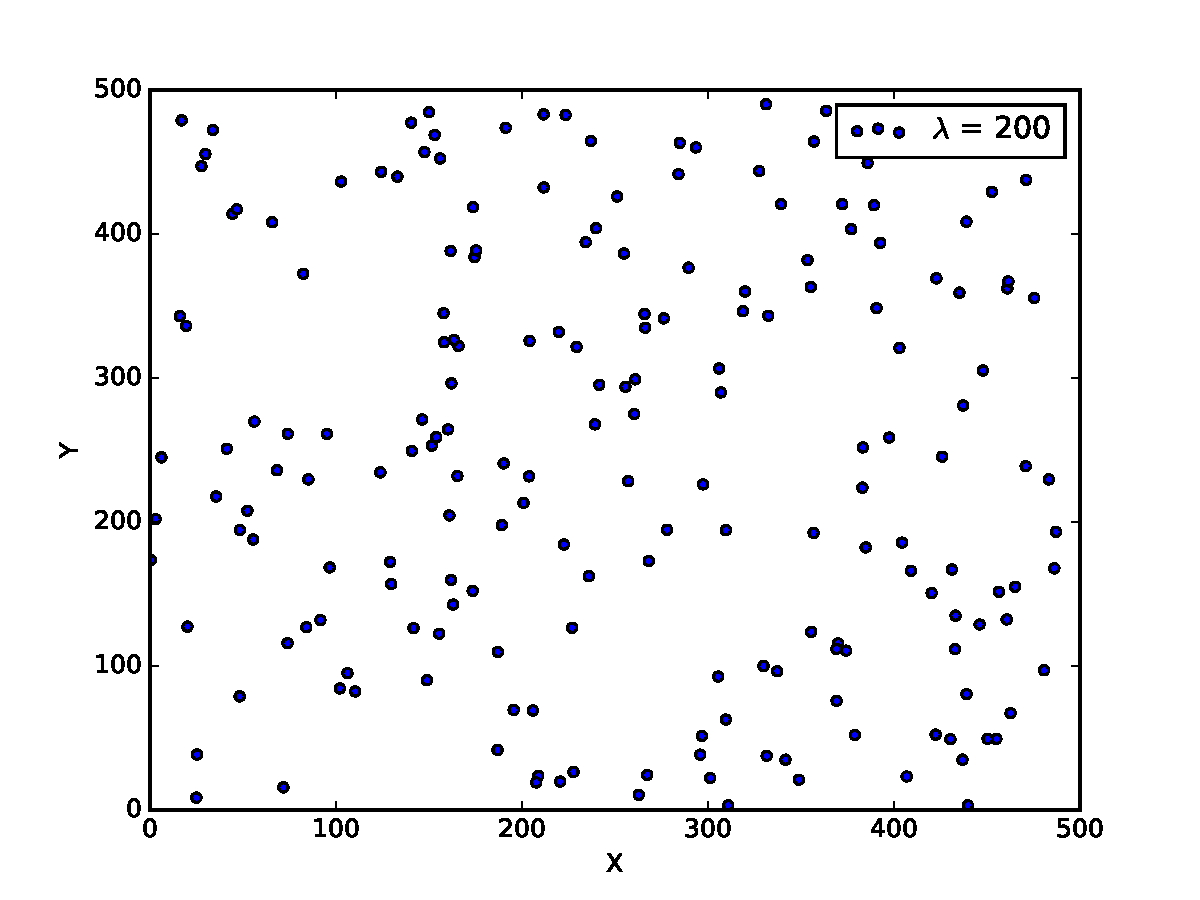
\includegraphics[scale = 0.6]{figures/PPP}
\caption{Example of a PPP with $\lambda = 200$}
\end{figure}

Thus we have generated the number and position of all our UEs according to a Poisson point process (PPP).

\section{Path loss (attenuation)} \label{PL}
Whenever transmission between devices is being investigated, loss due to attenuation as the signal propagates through space is an unavoidable topic. Distance degrades electromagnetic waves in terms of power in any real system and any simulation that does not reflect this phenomenon is simply not valid. 

In search of the best documented and most forward-looking models available, we settled on the use of METIS (Mobile and wireless communications Enablers for the Twenty-twenty Information Society), a EU Project that seeks to promote the definition of 5G mobile technologies. Its channel model, presented in its deliverables (\cite{Raschkowski}) was especially insightful. 

For the purposes of this thesis, the Stochastic Model, a ``geometry-based stochastic channel model'', was chosen for the way it lined up with our own goals, especially when it came to level of detail and complexity. Their figures are based on previous efforts by 3GPP studies to model these same phenomena. Due to the highly dense, urban system we are investigating, propagation scenario number one, ``Urban Micro'' was selected. Due to the constraints of this thesis, we narrowed our focus on Outside-to-Outside (020) connections, although the integration of Outside-to-Inside (O2I) could be a feature of future research.

When calculating the attenuation for a given path between two devices, there emerge two distinct cases, depending on whether there are any significant obstacles between the two of them: Line-of-sight (LOS) and Non-line-of-sight (NLOS).



\subsection{Manhattan grid} \label{mh_grid}
In order to determine whether a given link is a LOS or NLOS link, we need information about the obstacles present in the path between the two. In our case, we don't consider objects like cars and people explicitly, but rather account for all such minor objects and reflections they might create with a stochastic model (see \ref{SF}). Buildings, on the other hand, represent such massive, nigh-impenetrable objects that we must contemplate them concretely.

The preferred method mentioned in the METIS deliverables is the use of a ``Manhattan-like'' grid, meaning a city-layout comprised of rectangular blocks criss-crossed by wide streets. To determine both the size and the overall layout of our Manhattan Grid, we again turn to the extensive work done by METIS. The measurements with which their relevant models were tested were run in Madrid, with a grid of around 500 meters of both length and width. We homogenized the scenario by having exclusively square blocks, but maintained both the street width and the general dimensions.


\begin{table}[htbp]
\begin{center}
 \begin{tabular}{||p{3cm}|p{3cm}||} 
 \hline
 \textbf{Parameter} & \textbf{Value}\\
 \hline\hline
 Grid Dimensions & 500 m $\times$ 500 m \\ 
 \hline
 Block Width & 110 m \\
 \hline
 Block Length & 110 m \\
 \hline
 Street Width & 20 m \\
 \hline
\end{tabular}
\end{center}
\caption{Manhattan grid parameters}
\end{table}

The introduction of an explicit grid raises the issue of the positioning of our UEs again. Having scattered them in a Poisson point process (see \ref{PPP}), some inevitably now find themselves inside a building and not on the street, as is necessary for our O2O simulations. We overcome this obstacle by simply finding the shortest route from the position inside a block to the street: as the UE position is random, so too is the route taken. Thus we avoid completely discarding the randomness of their positioning. The results can be seen in figure \ref{fig:mh_grid_own} and compared to the actual city grid used for METIS measurements (figure \ref{fig:Madrid}).

\begin{figure}
\centering
\begin{subfigure}{.35\textwidth}
  \centering
  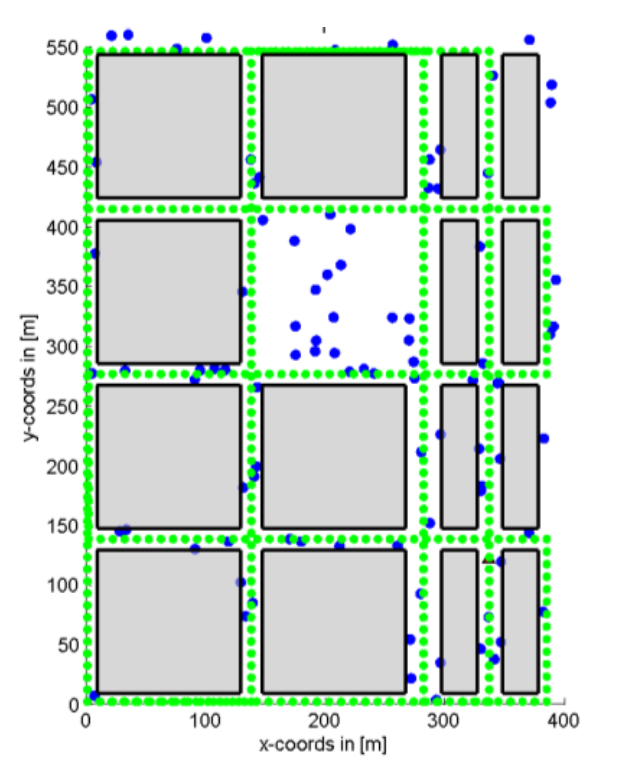
\includegraphics[width=1.2\linewidth]{figures/Madrid}
  \caption{Madrid grid \cite{Raschkowski}}
  \label{fig:Madrid}
\end{subfigure}%
\begin{subfigure}{.65\textwidth}
  \centering
  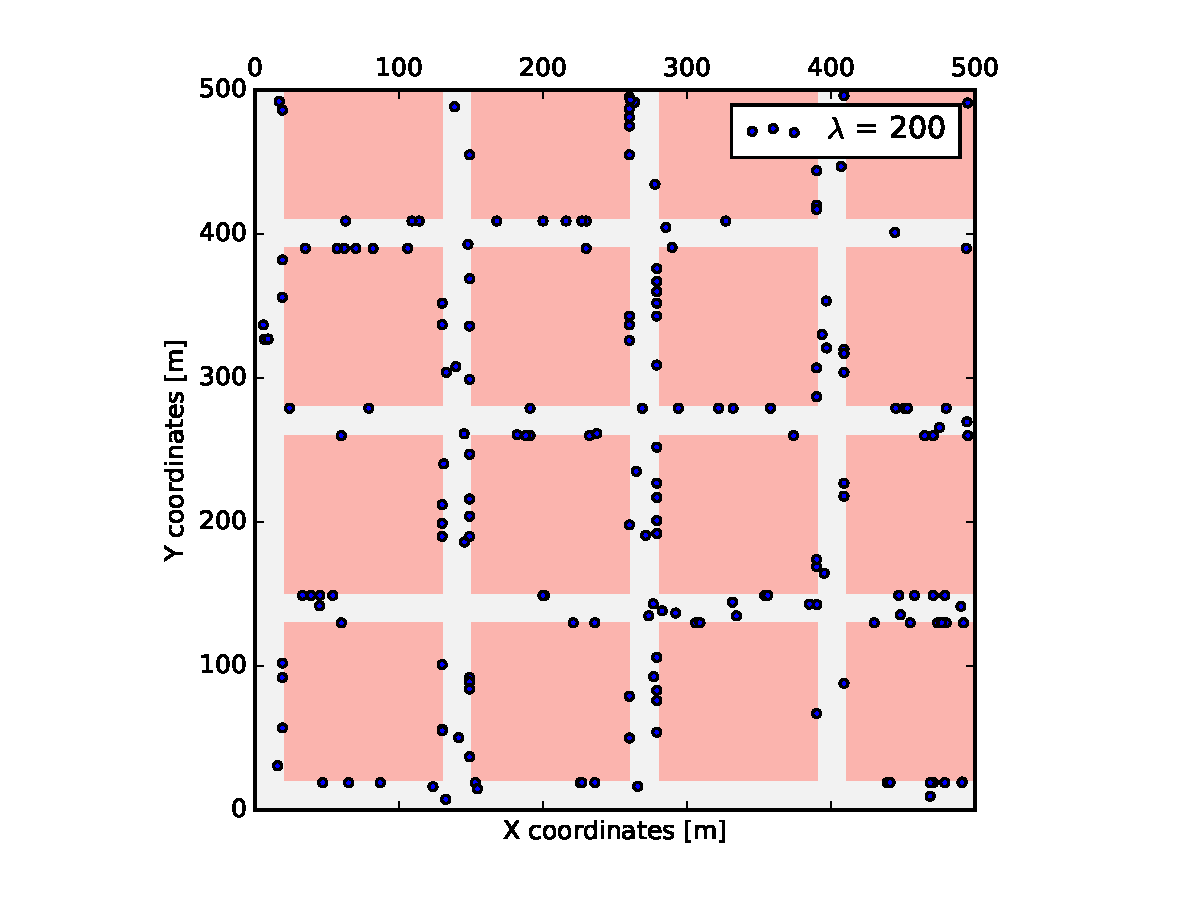
\includegraphics[width=1.058\linewidth]{figures/mh_grid}
  \caption{Own implementation, including moved UEs}
  \label{fig:mh_grid_own}
\end{subfigure}
\caption{Comparison between two Manhattan Grids}
\label{fig:mh_grid}
\end{figure}


With a Manhattan-like layout at the ready, questions about whether a link has LOS or not become much easier to answer.

\subsection{Line-of-sight} \label{LOS}
The overall model for pathloss used by \cite{Raschkowski} is derived specifically from the one presented in \cite{ReportITU-RM.2135-12009} by the ITU (International Telecommunication Union) and covers a wide frequency range (0.8 to 60 GHz). Distances between 10 and 500 meters are thus defined by two distinct equations, depending on whether the distance between the two points is greater than a certain ``breakpoint distance''. The distance $d^\prime_{BP}$ in question is defined by
\begin{equation} \label{eq:dbp}
d^\prime_{BP} = 0.87\, \exp\bigg( -\frac {log_{10} \big( \frac {f_c} {1GHz} \big)} {0.65} \,\bigg)\,\frac{4\,h^\prime_{BS}h^\prime_{UE}}{\lambda_{WL}}\,,
\end{equation}
with $h^\prime_{BS}$ as the effective height of the Base Station and $h^\prime_{UE}$ the effective height of the UE, with ``effective" denoting adjusting for environment height $h_e$. The $\lambda_{WL}$ is the wavelength of the signal, which is calculated from the center frequency $f_c$ and the speed of light $c$. It must be mentioned that for our transmissions, the height of both the origin and destination device will be identical more often than not, due to cluster connections being D2D links.

An additional ``pathloss offset'' $PL_1$ is defined in order to bring the model in agreement with the control measurements performed by METIS and is designed to account for elements like multipath fading.

\begin{equation} \label{eq:PL_1}
PL_{1|dB} = -1.38\,\log_{10}\,\bigg( \frac {f_c}{1Ghz} \bigg) + 3.34
\end{equation}


The actual pathloss equations are given as a function of distance $d$ by

\begin{equation} \label{eq:PL_LOS_1}
  PL_{LOS}(d)_{|dB} = 10\,n_1\,\log_{10}\bigg( \frac{d}{1m} \bigg) + 28.0 + 20 \log_{10} \bigg( \frac{f_c}{1GHz} \bigg) + PL_{1|dB}
\end{equation}
for $10\,m\,<\,d\, \le \,d^\prime_{BP}$ and
\begin{equation} \label{eq:PL_LOS_2}
  PL_{LOS}(d)_{|dB} = 10\,n_2\,\log_{10}\bigg( \frac{d}{d^\prime_{BP}} \bigg) + PL_{LOS}(d^\prime_{BP})_{|dB}
\end{equation}
for $d^\prime_{BP}\,<\,d\, \le \,500 m$ (compare with \cite{Raschkowski}). The parameters $n_1 = 2.2$ and $n_2 = 4.0$ are the power decay constant on both sides of the break point distance.

\subsection{Non-line-of-sight} \label{NLOS}
Most of the connections available to a given UE will be NLOS links. These happen whenever the UE tries to communicate with a device that is not on its same street and thus the signal has to travel a more convoluted way in order to be received. METIS defers explicitly to the final channel models, created by WINNER+ (Wireless World Initiative New Radio+) in \cite{Heino2010}. WINNER+ is a private consortium looking to further develop the IMT-A (International Mobile Telecommunications-Advanced) standards. 

The conceptual NLOS model in itself comes from an even earlier work, \cite{Meinila2009}, which details the relevant parameters for NLOS communication in an urban setting. In these cases, the corners resulting from intersecting streets act as relay nodes for the signal. \cite{Meinila2009} designates two distances needed to calculate the pathloss in this route, see figure \ref{fig:d1_d2}, where $d_1$ is distance from relay node to BS and $d_2$ to the UE. As was the case for the difference in heights between UE and BS, seeing as the links we are investigating are D2D, there is no real clear theoretical distinction between $d_1$ and $d_2$. However, we keep the distinction intact (with the same emitter/receiver relation) owing to the fact that ``[t]hough the pathloss between BS and UE must be the same regardless of the direction of signal transmission due to reciprocity, the pathloss \textit{models} do not necessarily hold the reciprocity'' (\cite{Raschkowski}).

\begin{figure}
\centering
\begin{subfigure}{.5\textwidth}
  \centering
  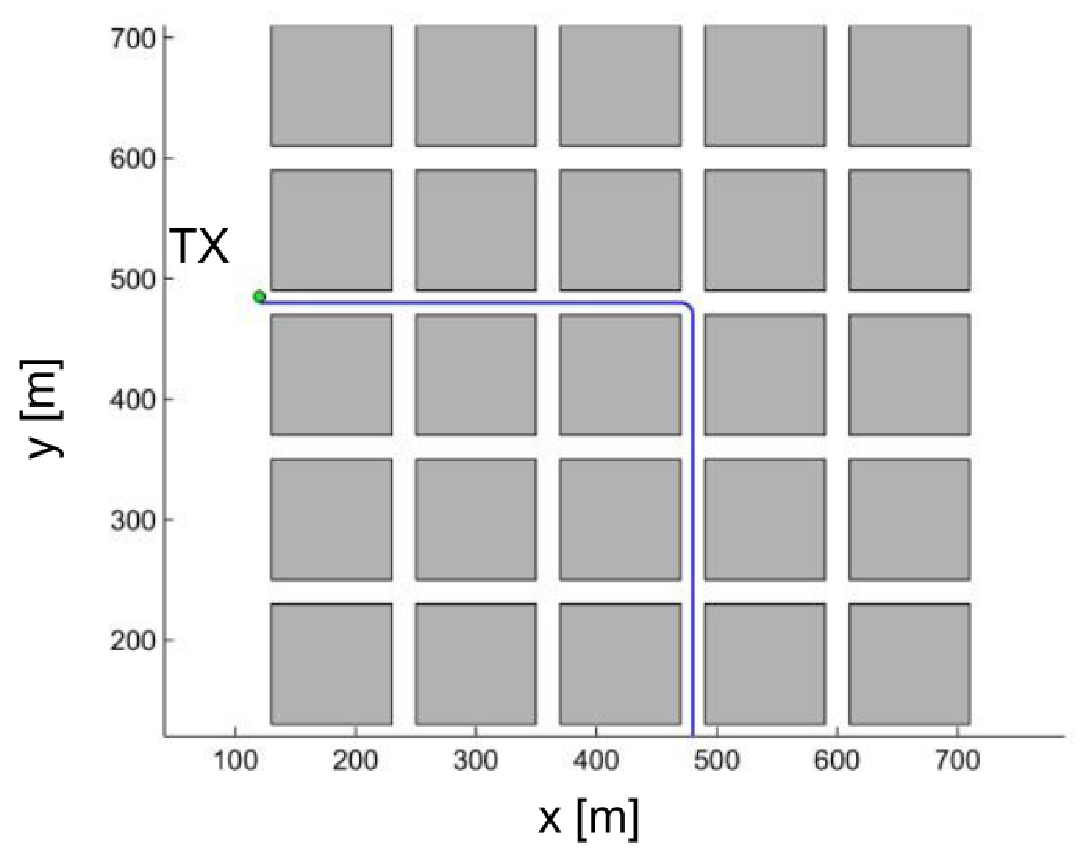
\includegraphics[width=1\linewidth]{figures/node_relay}
  \caption{Node Relay example \cite{Raschkowski}}
  \label{fig:node_relay}
\end{subfigure}%
\begin{subfigure}{.5\textwidth}
  \centering
  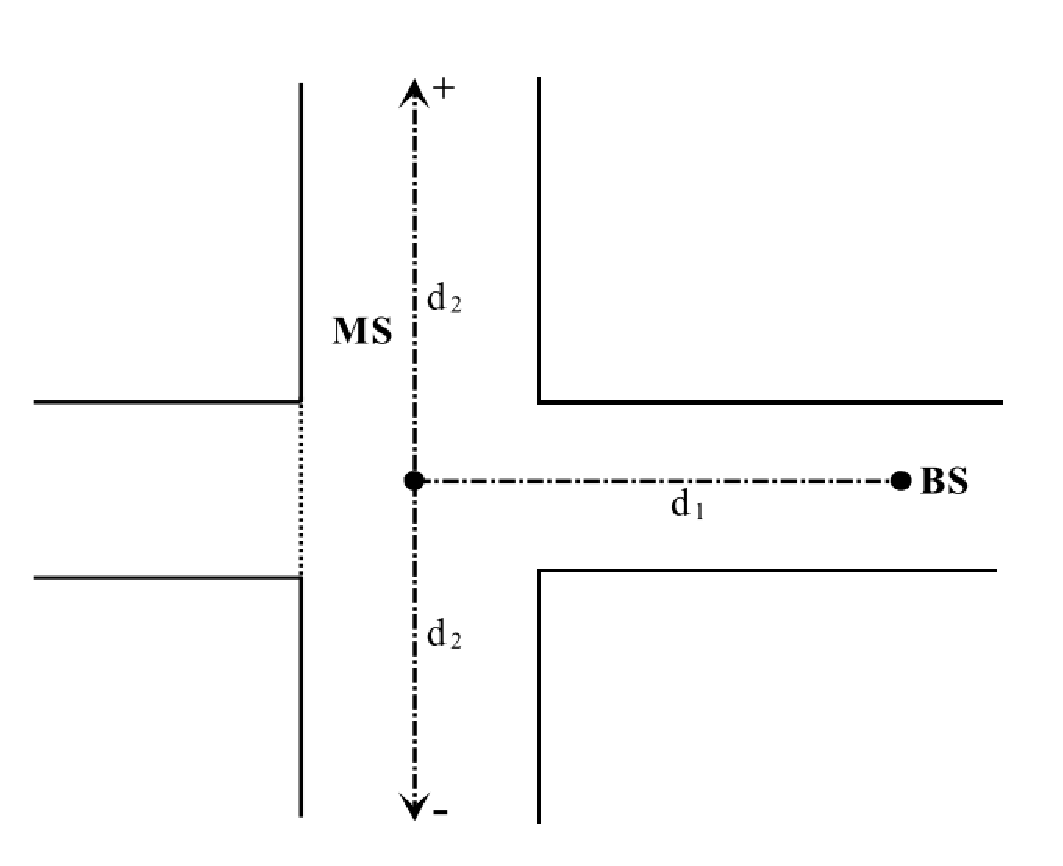
\includegraphics[width=1\linewidth]{figures/d1_d2}
  \caption{Distances $d_1$ and $d_2$ \cite{Meinila2009}}
  \label{fig:d1_d2}
\end{subfigure}
\caption{Calculation of NLOS path}
\label{fig:nlos_path}
\end{figure}

Thus, the formula for pathloss in the studied case is presented in \cite{Raschkowski} after a small simplification and again featuring the ``pathloss offset'' (equation \ref{eq:PL_1}) mentioned in \ref{LOS}:

%\begin{equation} \label{eq:NLOS}
\begin{equation} \label{eq:NLOS}
\begin{split}
  PL_{NLOS}(d_1,d_2)_{|dB} = & \,PL_{LOS}(d_1)_{|dB} + 17.9 - 12.5\,n_j \\
  & + 10\,n_j\,\log_{10} \bigg( \frac {d_2} {1 m} \bigg) + 3 \log_{10} \bigg( \frac { f_c } { 1 GHz } \bigg) + PL_{1|dB},
\end{split}
\end{equation}
where $n_j$ is a power decay constant calculated as

\begin{equation} \label{eq:n_j}
n_j = \max (2.8 - 0.0024\,d_1,\,1.84).
\end{equation}

In a rectangular Manhattan grid such as ours, a only two intersections are needed as relays in order to connect any two given points on the grid. An algorithm was thus created to calculate the shortest possible distance between the two devices using a maximum of two intersections. We take the shortest possible route because the signal spreads omni-directionally. An example of a calculated route between two points can be seen in figure \ref{fig:two_points}.

\begin{figure}[H]
\centering
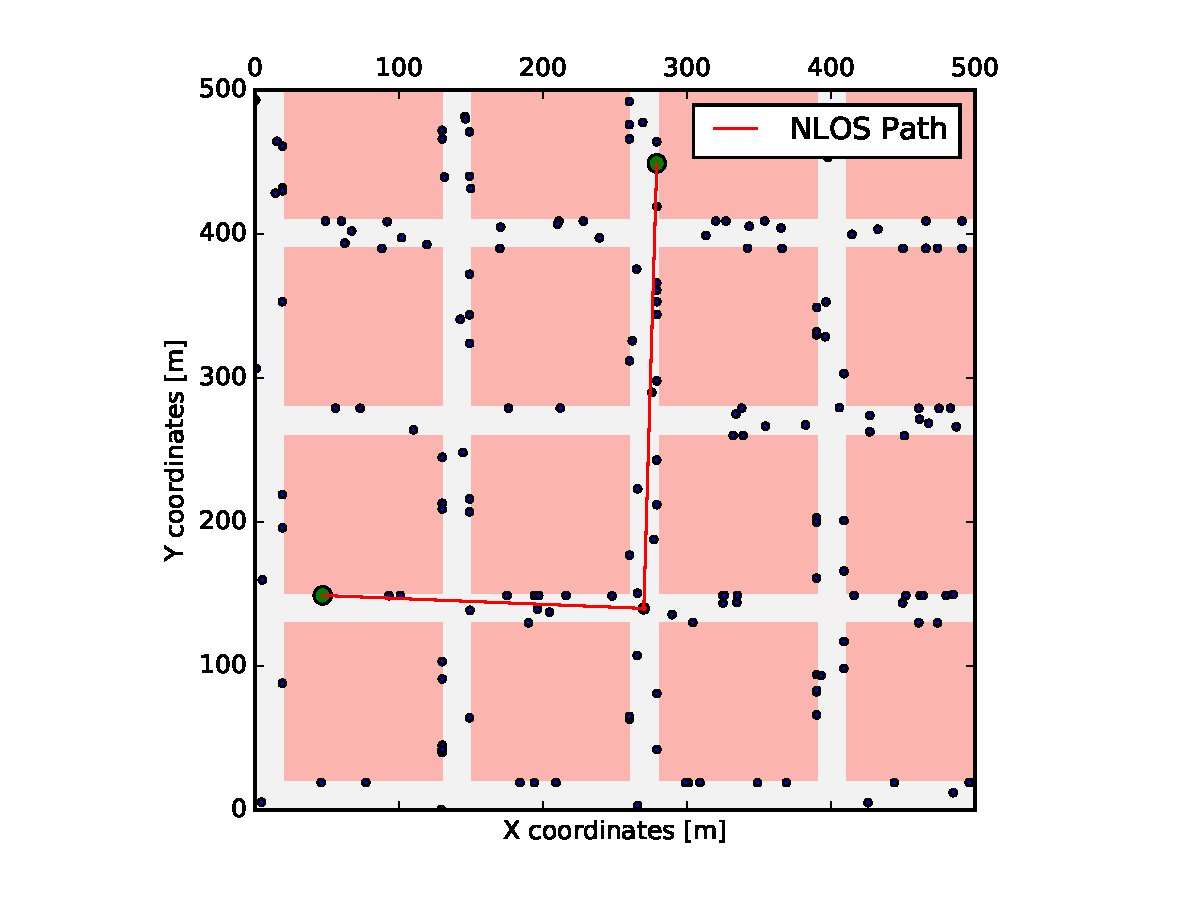
\includegraphics[width=.7\linewidth]{figures/two_points}
\caption{Visualization of NLOS path with intersection acting as relay node}
\label{fig:two_points}
\end{figure}

\section{Shadow fading} \label{SF}
As mentioned in \ref{mh_grid}, Shadow Fading - meaning the effects on the signal caused by smaller obstacles - as well as the reflections they create are modelled through a stochastic model. This type of fluctuation, called ``Shadow Fading'' or ``long-term fading'' is often realized through a Gaussian distribution in the logarithmic scale (also called a log-normal distribution), as asserted in \cite{Forkel2004} and shown below in its probability density function. In our case, we followed METIS specifications and set $\mu_{L_s} = 0$ and $\sigma_{L_s} = 7 \text{dB}$.

\begin{equation} \label{eq:SF}
p(L_s) = \frac{1}{{\sigma_{L_s} \sqrt {2\pi } }}\,\exp\bigg(-\frac{(L_s - \mu_{L_s})^2}{2\,\sigma_{L_s}^2}\bigg)
\end{equation}

While any given point is distributed randomly along the normal distribution, completely random and uncorrelated shadow fading variables make little sense when one considers that the effects of any given set of obstacles won't change much in the space of a couple of meters. In order to account for the necessary correlation that these shadow fading variables experience, a normalized autocorrelation function is introduced, both in \cite{Forkel2004} and \cite{Raschkowski}, with a decorrelation value suggested by METIS $d_{corr} = 8 m$.

\begin{equation} \label{eq:corr}
R(\Delta x) = \exp\bigg(-\frac{|\Delta x|}{d_{corr}}\,\ln(2)\bigg)
\end{equation}

After generating the shadow fading variables with equation \ref{eq:SF} and the autocorrelation coefficients with equation \ref{eq:corr}, both matrices are convoluted to generate the correlated values. Convolution does not alter the underlying distribution, but it does elicit a correction of the mean and standard deviation (compare with \cite{Forkel2004}) in order to return it to the values of the original Gaussian distribution. Our realization is shown below, both before and after the aforementioned correction for spatial correlation.

%\centering
\begin{figure}
\centering
\begin{subfigure}{.5\textwidth}
  \centering
  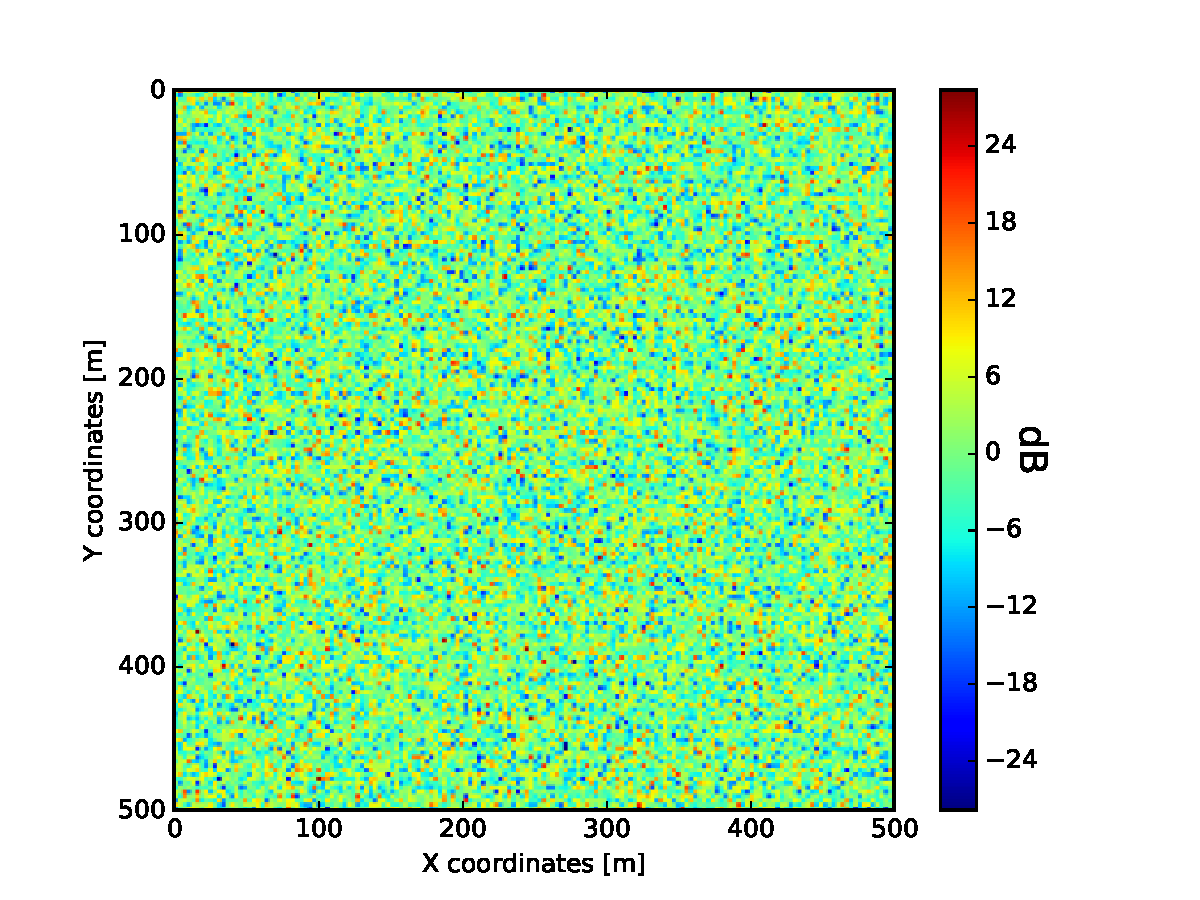
\includegraphics[width=1.1\linewidth]{figures/noise_before}
  \caption{Uncorrelated Shadow Fading values}
  \label{fig:sf_no_correlation}
\end{subfigure}%
\begin{subfigure}{.5\textwidth}
  \centering
  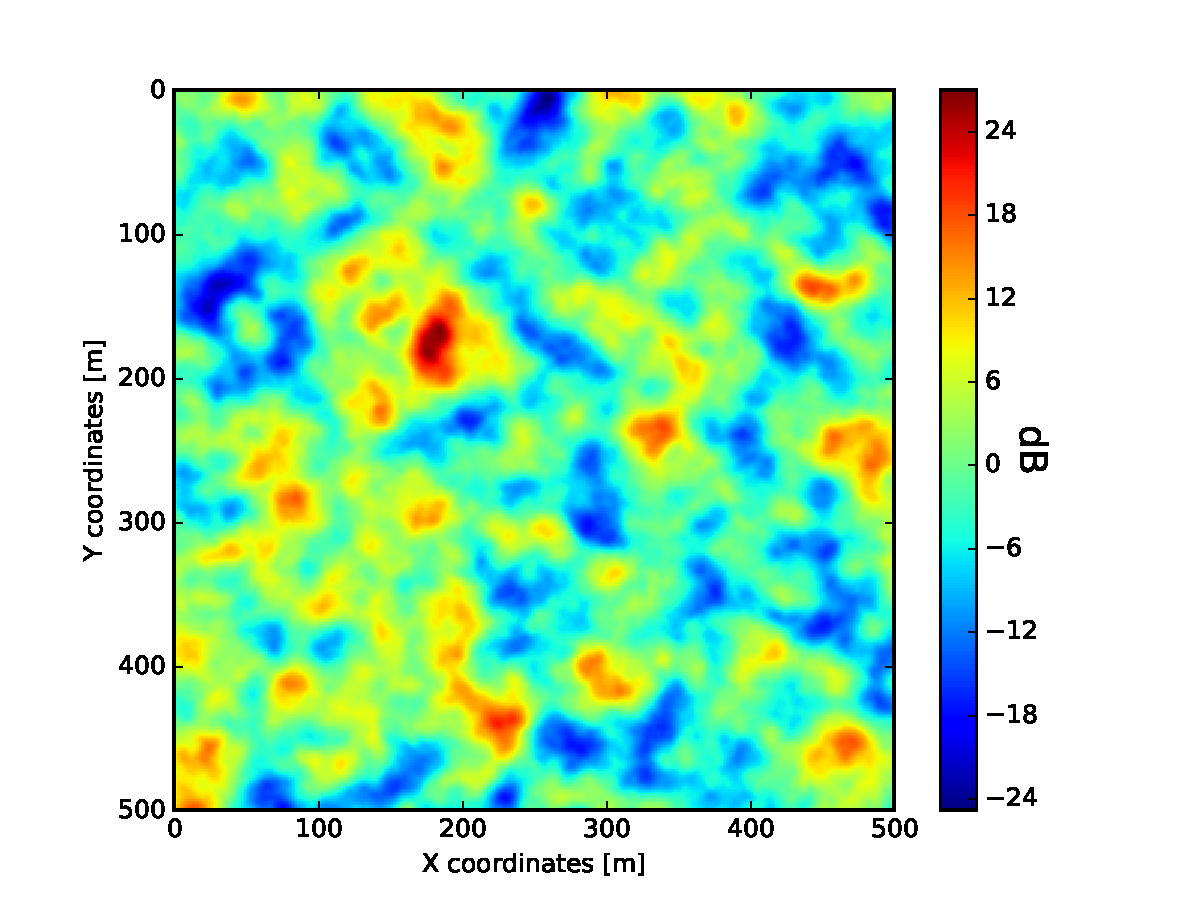
\includegraphics[width=1.1\linewidth]{figures/noise_after}
  \caption{Correlated Shadow Fading values}
  \label{fig:sf_correlated}
\end{subfigure}
\caption{Shadow Fading values before and after correlation adjustment}
\label{fig:SF}
\end{figure}


These shadow fading fading values are added to the pathloss values in order to fully account for all the obstacles in the way of the signal between two devices. The complete attenuation value then determines the received signal strength at the target device.

A summary of the relevant parameters utilized for the calculation of the pathloss can be seen in table \ref{tbl:PL}

\begin{table}[H]
\begin{center}
 \begin{tabular}{||p{7cm}|p{2.5cm}||} 
 \hline
 \textbf{Parameter} & \multicolumn{1}{|c||}{\textbf{Value}}\\
 \hline\hline
 Mean point density $\lambda$ & \multicolumn{1}{|c||}{$50 - 1000$} \\ 
 \hline
 Center Frequency $f_c$& \multicolumn{1}{|c||}{$2\,\text{GHz}$} \\
 \hline
 Wavelength $\lambda_{WL}$ & \multicolumn{1}{|c||}{$0.15\,\text{m}$}\\
 \hline
 Speed of light $c$ & \multicolumn{1}{|c||}{$3 \cdot 10^8\,\frac{\text{m}}{\text{s}}$}\\
 \hline
 Height of UE $h_{UE}$ & \multicolumn{1}{|c||}{$1.5\,\text{m}$} \\
 \hline
 Height of BS $h_{BS}$ & \multicolumn{1}{|c||}{$10\,\text{m}$} \\
 \hline
 Environment height $h_e$ & \multicolumn{1}{|c||}{$1\,\text{m}$} \\
 \hline
 Power decay constant $n_1$ & \multicolumn{1}{|c||}{$2.2$}\\
 \hline
 Power decay constant $n_2$ & \multicolumn{1}{|c||}{$4.0$}\\
 \hline
 Shadow Fading mean $\mu_{L_s}$ &\multicolumn{1}{|c||}{$0$} \\
 \hline
 Shadow Fading standard deviation $\sigma_{L_s}$ & \multicolumn{1}{|c||}{$7\,\text{dB}$}\\
 \hline
 Decorrelation distance $d_{corr}$ &\multicolumn{1}{|c||}{$8\,\text{m}$}\\
 \hline
\end{tabular}
\end{center}
\caption{Parameters relevant for pathloss calculation}
\label{tbl:PL}
\end{table}

\section{Random access procedure and interference} \label{RAP}
When reducing the load that the eNB experiences as a result of an increase in the amount of devices connecting to it by means of clustering, a large amount of the load is simply transferred to the cluster heads. These have then to take up the functions of the eNB in terms of implementing a random access procedure through which to service the UEs connecting to it. As mentioned in section \ref{B:D2D}, we contemplate an explicit separation of resources for normal BS to UE communication and D2D communication, putting further constraints on the ability of the cluster head to detect and separate signals using the same resource blocks. In order to best model these kinds of phenomena, the author utilized simulations developed by his supervisor, M.Sc. Mikhail Vilgelm, that were kindly put at his disposition for this work.

Firstly, a Poisson process is used in modeling the arrival of packages proceeding from connected UEs to the appropriate cluster head. This Poisson arrival process is analogous to that shown in equation \ref{eq:Poisson} and yields the amount of packages arrived at a certain point in time instead of points in an area. The arrival rate, $\lambda_A$ was set by recommendation of the author's supervisor to a level where the derivative of the throughput with respect to the arrival rate is positive, at $\lambda_A = 1.5$.

The requests are generated at the given rate and broadcast with a set transmission power $P_{Tx}$. Although there are many proposals for power control schemes in D2D communications, such as \cite{Erturk2013}, \cite{Wei2012} or \cite{Lee}, due to there being so many varied schemes and them adding such complexity to the simulation, it was decided that power control would not be part of the scope of this work. As in \cite{Klugel2014a}, we decide to use $P_{Tx} = 23\,\text{dBm}$ for our simulation, which is incidentally the power level used for coverage issue identification in \cite{3rdGenerationPartnershipProject;2012} and the maximum transmit power for public safety defined in \cite{3rdGenerationPartnershipProject;}, both by the 3GPP.

The power is then affected by the appropriate attenuation at the spot of the receiving device (see section \ref{PL}) and the resulting power is the received power $P_{Rx|dBm} = P_{Tx|dBm} - PL_{|dB}$. In order to assess whether a given signal has reached the cluster head with enough power to be detected, we look at the SINR (Signal-to-Interference-and-Noise-Ratio) of the transmission. For the calculation of the noise we use a thermal noise density $N_0 = -174\,\frac{\text{dBm}}{\text{Hz}}$, UE receiver noise figure $NF_{UE} = 9\,\text{dB}$ and system bandwidth $W = 10\,\text{MHz}$, as defined in \cite{3rdGenerationPartnershipProject;2012}. 

The incoming requests are checked for additional interference coming from other requests using the same preamble, both within and without the cluster. The received power $I$ of those interfering signals at the cluster head are added and that total added to the noise power $P_N$ to finally calculate the SINR, see equation \ref{eq:SINR}. As mentioned earlier, the available preambles for transmission of a D2D link are drawn from the overall pool of preambles available in LTE-A. As mentioned in \cite{Cox2012}, 64 preambles are available to the cell, only 6 of which are available for D2D communication. This is to allow normal cellular UEs to experience an acceptable QoS (Quality of Service), while still allowing other devices access to the network.

\begin{equation}\label{eq:SINR}
SINR = \frac {P_{Rx}} {I + P_N}
\end{equation}

As to the minimum SINR needed to connect to the cluster head, a threshold of $SINR_{thr} = 10\,\text{dB}$ was chosen within the range presented in \cite{3Gpp2009} for the minimum ratio necessary to transmit with ``an acceptably low BER (Bit Error Rate) in the output data.'' Those requests under the threshold will be filtered out before they are dealt with by the cluster head. Please note that although they are not counted towards successful requests, they will count towards interference values of other requests that may or may not clear the threshold.

Finally, requests clearing the threshold will be handled by the cluster head, who will then check for intra-cluster preamble collisions and give feedback, negative or positive, to the UEs. For simplicity's sake, feedback is assumed to arrive safely back at the UE; positive feedback elicits no action from the original transmitter. Upon reception of negative feedback, on the other hand, the UE ``backs off'' for an amount of time before attempting the connection once again at a later point in time. If the device is told to back off 20 times, it assumes the connection has failed completely and will not try again until another packet is generated at that UE. The time for each slot was set at $10\,\text{ms}$, while the overall simulation duration was put at $5\,\text{s}$.

Readers can find a summary of all used parameters for this stage on table \ref{tbl:RA}.

\begin{table}[H]
\begin{center}
 \begin{tabular}{||p{10cm}|p{2.5cm}||} 
 \hline
 \textbf{Parameter} & \multicolumn{1}{|c||}{\textbf{Value}}\\
 \hline\hline
 Request arrival rate $\lambda_A$ & \multicolumn{1}{|c||}{$1.5$} \\ 
 \hline
 Transmission power $P_{Tx}$& \multicolumn{1}{|c||}{$23\,\text{dBm}$} \\
 \hline
 Noise density $N_0$ & \multicolumn{1}{|c||}{$-174\,\frac{\text{dBm}}{\text{Hz}}$}\\
 \hline
 UE receiver noise figure $NF_{UE}$ & \multicolumn{1}{|c||}{$9\,\text{dB}$}\\
 \hline
 BS receiver noise figure $NF_{BS}$ & \multicolumn{1}{|c||}{$5\,\text{dB}$} \\
 \hline
 System Bandwidth $W$ & \multicolumn{1}{|c||}{$10\,\text{MHz}$} \\
 \hline
 Number of total LTE-A preambles & \multicolumn{1}{|c||}{$64$} \\
 \hline
 Number of preambles available for D2D communication& \multicolumn{1}{|c||}{$6$}\\
 \hline
 SINR threshold $SINR_{thr}$ & \multicolumn{1}{|c||}{$10\text{dB}$}\\
 \hline
 Slot duration & \multicolumn{1}{|c||}{$10\,\text{ms}$}\\
 \hline
 Total duration &\multicolumn{1}{|c||}{$5\,\text{s}$}\\
 \hline
\end{tabular}
\end{center}
\caption{Parameters relevant for random access and interference}
\label{tbl:RA}
\end{table}

The last piece of the puzzle is, of course, the actual mapping of UEs to cluster heads. These are fed into the random access and interference simulation by the clustering algorithms.

\section{Clustering Algorithms}
Clustering algorithms determine which UEs will be connected to which cluster heads, as well as which UEs will turn into cluster heads in the first place. Because of the nature of our research (regarding D2D communication), we eschewed any schemes that required dedicated gateways into the networks. In the definition of the scope of this work, we also decided to leave out any algorithms with multi-hop possibilities, simply due to the sheer complexity that would have represented. Algorithms presented here thus feature only one aggregation stage at the cluster head, which then forwards the data to the eNB.

Most of the work done in clustering algorithms for wireless networks comes from the area of Wireless Sensor Networks (WSN), where large amounts of sensor nodes form a network communicating with a central unit of control. These types of structures lend themselves especially to grouping and aggregation, considering especially that there is often a lot of redundancy in the collected data. Energy efficiency and resilience of networks is often of paramount importance, in an attempt to minimize maintenance overhead. There have been several studies about clustering algorithms in this area, such as \cite{Jiang2009} or \cite{Afsar2014}. 

Looking toward WSNs seems like the closest logical step when considering D2D communications, but an effort was also made to look at algorithms not native to WSNs.